\section{Increasing System Performance}

\begin{center}
    \begin{tabular}{|l|l|}
    \hline
    Speed vs Low Power &  \\
    Aspects of Optimization &  \\
    \hline
    Optimizing for & Drawbacks on \\
    \hline
    Higher speed & Power, cost, chip area \\
    \hline
    Lower cost & Speed, reliability \\
    \hline
    Zero power consumption & Speed, cost \\
    \hline
    Super reliable & Chip area, cost, speed \\
    \hline
    Temperature range & Power, cost lifetime \\
    \hline
    \end{tabular}
    \end{center}
    
    \section*{RISC = Reduced Instruction Set Computer}
    \begin{itemize}
      \item Few instructions, unique instruction format
      \item Fast decoding, simple addressing
      \item Less hardware -> allows higher clock rates
      \item More chip space for registers (up to 256!)
      \item Load-store architecture reduces memory access,
    \end{itemize}
    
    CPU works at full-speed on registers
    
    \begin{itemize}
      \item Higher clock frequencies
      \item Easy and shorter pipelines (instructio size / duration)\\
    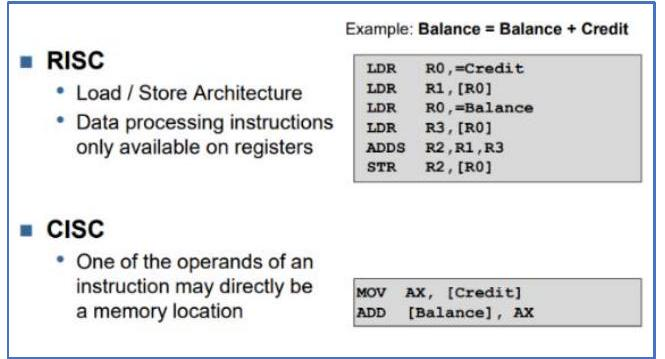
\includegraphics[width=\linewidth]{images/2024_12_29_79e6b22f503fb7b4f718g-13(1)}
    \end{itemize}
    
    CISC = Complex Instruction Set Computer
    
    \begin{itemize}
      \item More complex and more instructions
      \item Less program memory needed with complex instructions
      \item Short programs may work faster with less memory accesses
    \end{itemize}
    
    \section*{Von Neuman Arhcitecture}
    \begin{itemize}
      \item Same memory holds program and data
      \item $\quad$ Single bus system between CPU and memory Systembus\\
    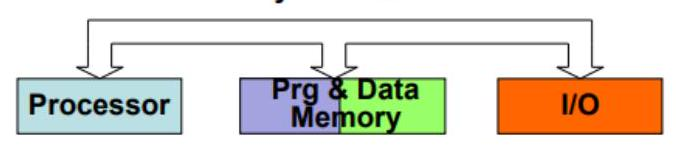
\includegraphics[width=\linewidth]{images/2024_12_29_79e6b22f503fb7b4f718g-13}
    \end{itemize}
    
    \section*{Harvard Architecture}
    \begin{itemize}
      \item «Mark I» at Harvard University
      \item Separate memories for program and data
      \item Two sets of addresses/data buses between CPU and memory\\
    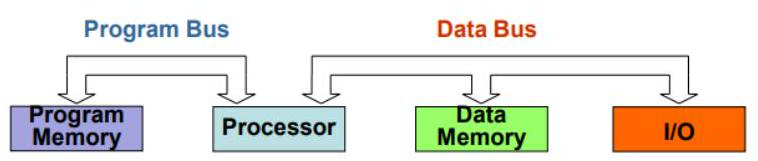
\includegraphics[width=\linewidth]{images/2024_12_29_79e6b22f503fb7b4f718g-13(2)}
    \end{itemize}
    
    How to Increase System Speed?\\
    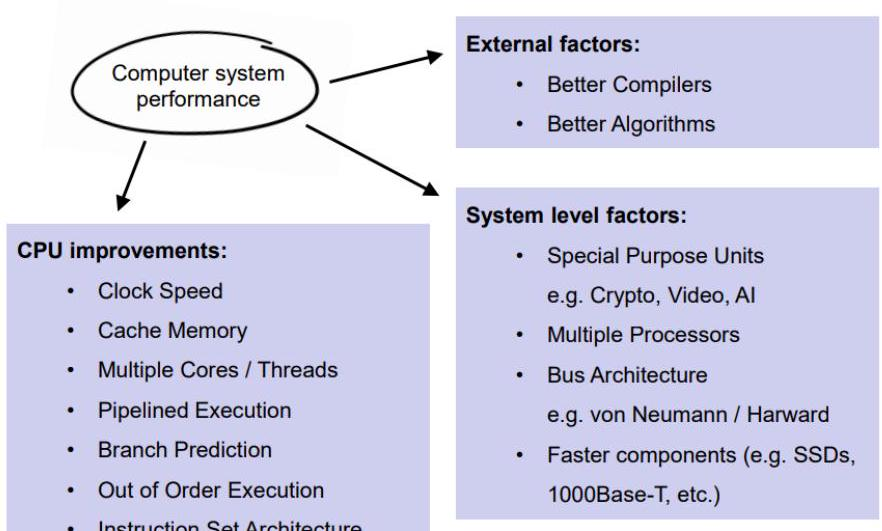
\includegraphics[width=\linewidth]{images/2024_12_29_79e6b22f503fb7b4f718g-13(3)}
    
    Fetching the next instruction, while the current one decodes\\
    Sequential vs. Pipelined\\
    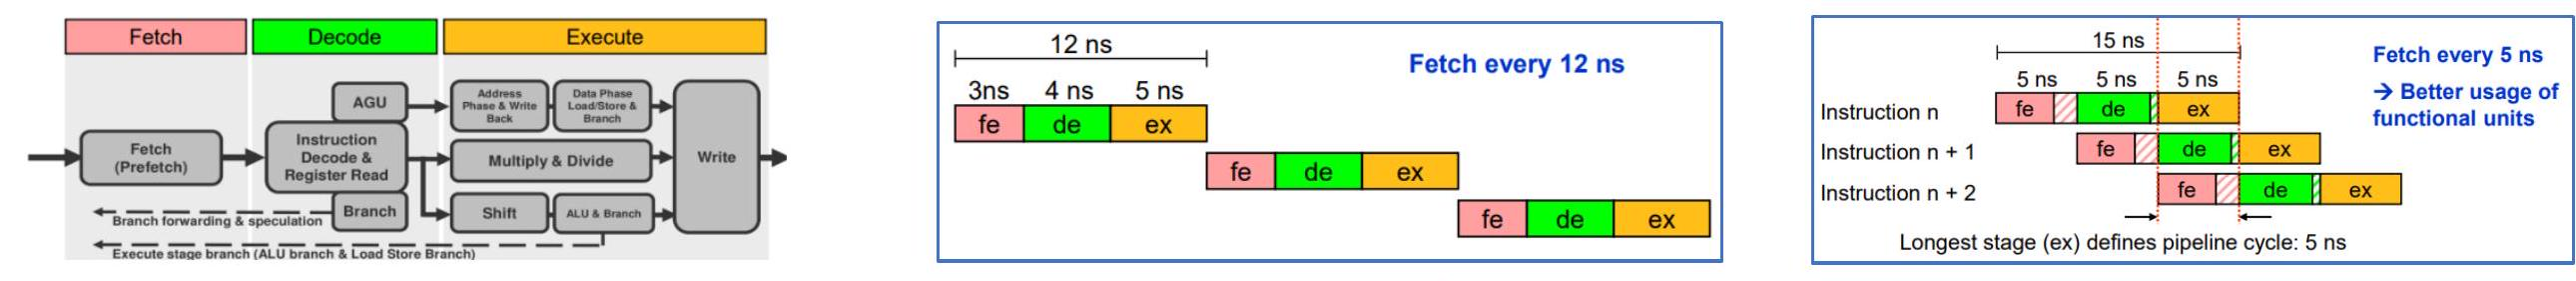
\includegraphics[width=\linewidth]{images/2024_12_29_79e6b22f503fb7b4f718g-14(2)}
    
    \section*{Timings and definitions (Example)}
    \begin{itemize}
      \item Fe: fetch Read instructions 3 ns
      \item De: decode Decode instruction, read register or memory 4 ns
      \item Ex: execute Execute instruction, write back result 5 ns\\
    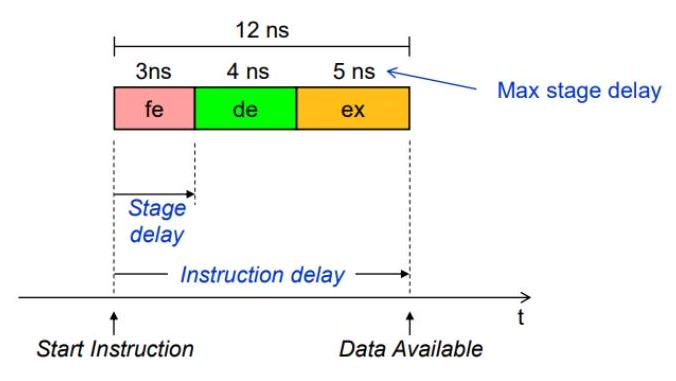
\includegraphics[width=\linewidth]{images/2024_12_29_79e6b22f503fb7b4f718g-14(1)}
    \end{itemize}
    
    \section*{Advantages of pipelining}
    \begin{itemize}
      \item All stages are set tot he same execution time
      \item Massive performance gain
      \item Simpler hardware at each stage allows for a higher clock rate
    \end{itemize}
    
    \section*{Disadvantages}
    \begin{itemize}
      \item A blocking stage blocks while pipeline
      \item Multiple stages may need to have access to the memory at the same time
    \end{itemize}
    
    \section*{Instructions per second}
    Without pipelining
    
    $$
    \frac{\text { Instructions }}{\text { second }}=\frac{1}{\text { Instruction delay }}
    $$
    
    With pipelining
    
    \begin{itemize}
      \item Pipeline needs to be filled first
      \item After filling, instructions are executed after every stage
    \end{itemize}
    
    $$
    \frac{\text { Instructions }}{\text { second }}=\frac{1}{\text { Max stage delay }}
    $$
    
    \section*{Optimal pipelining}
    \begin{itemize}
      \item All operations here are on registers
      \item In this example it takes 6 clock cycles to execute 6 instructions
      \item $\quad$ Clock cycles per instruction (CPI) = 1\\
    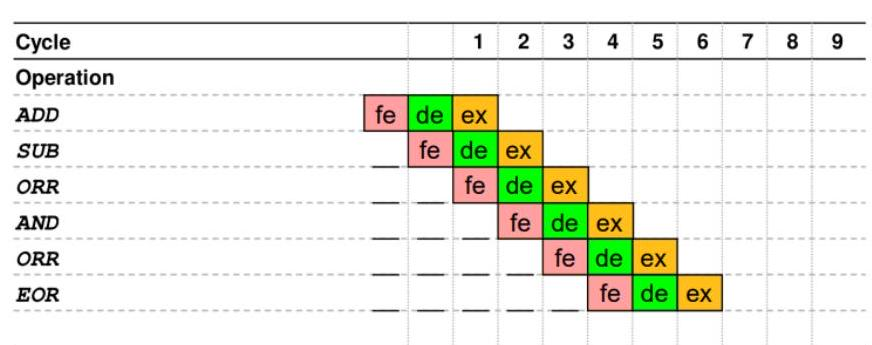
\includegraphics[width=\linewidth]{images/2024_12_29_79e6b22f503fb7b4f718g-14}
    \end{itemize}
    
    \section*{Special situation: LDR}
    \begin{itemize}
      \item In this example it takes 7 clock cycles to execute 6 instructions
      \item Read cycle must complete on the bus before LDR instruction can complete
      \item Next 2 instructions must wait one pipeline cycle ( $\mathrm{S}=$ stall)
      \item Clock cycles per Instruction (CPI) $=1.2$
    \end{itemize}
    
    \section*{Control Hazards}
    \begin{itemize}
      \item Branch / jump decisions occur in stage 3 (ex)
      \item Worst case scenario - conditional branch taken:\\
    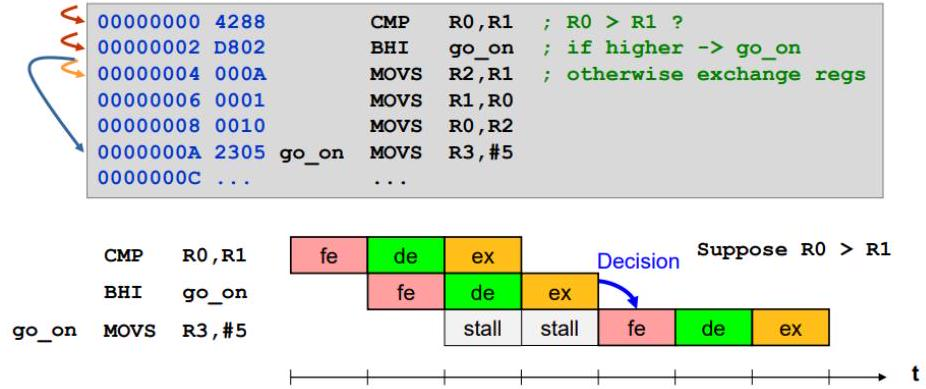
\includegraphics[width=\linewidth]{images/2024_12_29_79e6b22f503fb7b4f718g-15}
    \end{itemize}
    
    \section*{Reduce control hazards}
    \begin{itemize}
      \item Loop fusion reduces control hazards
    \end{itemize}
    
    \section*{Ideas to further improve pipelining}
    \begin{itemize}
      \item Branch prediction
      \item Store last decisions made for each conditional branch
      \item -> probability is high that the same decision is taken again
      \item Instruction prefetch
      \item Fetch several instructions in advance
      \item -> better use of system bus
      \item -> possibility of «Out of Order Execution»
      \item Out of Order Execution
      \item If one instruction stalls, it might be possible to already execute the next instruction
    \end{itemize}
    
    \section*{Limits of optimization}
    \begin{itemize}
      \item Complex optimizations -> sever security problems
      \item Instructions executed, that would throw access violations under «In Order» circumstances.
      \item «Meltdown» and «Spectre» attacks: allow a process to access the data of another process
    \end{itemize}
    
    \section*{Parallel Computing}
    \begin{itemize}
      \item Streaming / Vector processing One instruction processes multiple data items simultaneously
      \item Multithreading Multiple programs/threads share a single CPU
      \item Multicore Processors One processor contains multiple CPU cores
      \item Multiprocessor Systems A computer system contains multiple processors
    \end{itemize}